\documentclass[11pt,fleqn]{article} % Default font size and left-justified equations

%\usepackage{standalone}

\usepackage{todonotes}
\usepackage{color}
% use \todo{note} OR \missingfigure{Add my picture here}

\usepackage[top=3cm,bottom=3cm,left=3.2cm,right=3.2cm,headsep=10pt,a4paper]{geometry} % Page margins
\usepackage{xcolor} % Required for specifying colors by name
\definecolor{ocre}{RGB}{243,102,25} % Define the orange color used for highlighting throughout the book


% Font Settings


% SLG commented out


% \usepackage{avant} % Use the Avantgarde font for headings
%\usepackage{times} % Use the Times font for headings
% \usepackage{microtype} %Slightly tweak font spacing for aesthetics
% \usepackage{mathptmx} % Use the Adobe Times Roman as the default text font together with math symbols from the Sym­bol, Chancery and Com­puter Modern fonts


%  \usepackage[scaled=0.90]{couriers} %What is this used for?




% SLG commented out
% \def\thereforesymbol{
% \leavevmode
% \lower0.1ex\hbox{$\cdot$}
% \kern-0.2em\raise0.7ex\hbox{$\cdot$}
% \kern-0.2em\lower0.2ex\hbox{$\cdot$}
% \thinspace}


% \usepackage{CJKutf8}
%For cyrillic characters  (do we have any?)


% slg commented this out:
% \usepackage[OT2,T1]{fontenc}
% \DeclareSymbolFont{cyrletters}{OT2}{wncyr}{m}{n}
% \DeclareMathSymbol{\Sha}{\mathalpha}{cyrletters}{"58}


\usepackage[T1]{fontenc}
\usepackage[section]{placeins}

% slg commented these out:
% \usepackage{amssymb}
 \usepackage{fancyvrb}
%  \usepackage{color}




%define a verbatim text for bold user input
\newcommand\verbbf[1]{\textbf{$\blacksquare$ #1}}
%define a verbatim text without box in front
\newcommand\verbbnbf{\textbf}


\PassOptionsToPackage{hyphens}{url}


\usepackage[pdftitle={Programmers Manual for Developing Bulk Extractor Scanner Plug-ins},
              pdfauthor={Jessica R. Bradley, Simson L. Garfinkel},
              pdfkeywords={bulk extractor, scanners, plug-ins, bulk extractor developers}]{hyperref}
\makeatletter
\g@addto@macro{\UrlBreaks}{\UrlOrds}
\makeatother
% \usepackage{microtype} % Slightly tweak font spacing for aesthetics
%\usepackage[utf8]{inputenc} % Required for including letters with accents
\usepackage[T1]{fontenc} % Use 8-bit encoding that has 256 glyphs




%\usepackage[a4paper,pdftex]{geometry}                                                                                % A4paper margins
\setlength{\oddsidemargin}{5mm}                                                                                                % Remove 'twosided' indentation
\setlength{\evensidemargin}{5mm}


\usepackage[english]{babel}
%\usepackage[protrusion=true,expansion=true]{microtype}        
\usepackage{amsmath,amsfonts,amsthm,amssymb}
\usepackage{graphicx}


\usepackage{tabularx}


% Simson commented this out:
%use autoref or Autoref for lowercase or uppercase beginning of references
\usepackage{catoptions}
\makeatletter
\def\figureautorefname{figure}
\def\tableautorefname{table}
\def\Autoref#1{%
  \begingroup
  \edef\reserved@a{\cpttrimspaces{#1}}%
  \ifcsndefTF{r@#1}{%
    \xaftercsname{\expandafter\testreftype\@fourthoffive}
      {r@\reserved@a}.\\{#1}%
  }{%
    \ref{#1}%
  }%
  \endgroup
}
\def\testreftype#1.#2\\#3{%
  \ifcsndefTF{#1autorefname}{%
    \def\reserved@a##1##2\@nil{%
      \uppercase{\def\ref@name{##1}}%
      \csn@edef{#1autorefname}{\ref@name##2}%
      \autoref{#3}%
    }%
    \reserved@a#1\@nil
  }{%
    \autoref{#3}%
  }%
}
\makeatother


\usepackage{amsmath}


\usepackage{booktabs}


% slg commented out:
% \usepackage{makecell}


\usepackage{color}
\usepackage{graphicx}
%\usepackage {hyperref}
\usepackage{listings}
\usepackage{xspace}


% slg commented out:
\usepackage[toc, page]{appendix}
\usepackage[labelfont=bf]{caption}
%http://tex.stackexchange.com/questions/27663/using- bold-italic-text-inside-listings


% slg commented out:
% \usepackage{multirow} %for multirow tables




\newcommand{\HRule}{\rule{\linewidth}{0.5mm}}
\usepackage{fancyhdr}


\usepackage{array}



\setcounter{secnumdepth}{5}
\setcounter{tocdepth}{5}
 
%\usepackage{arabtex}

\usepackage{verbatim}

\raggedbottom

\begin{document}

%define macros for commonly used terms that require special formatting
\newcommand \sscope {\textit{SectorScope}\xspace}
\newcommand \hdb {\textit{hashdb}\xspace}
\newcommand \aut {\textit{Autopsy}\xspace}

\hypersetup{%
    pdfborder = {0 0 0}
}

\lstdefinestyle{customfile}{
basicstyle=\footnotesize\ttfamily, frame=single, float=htpb}

\begin{titlepage}





% LaTeX Template: Titlepage
% This is a title page template which be used for both articles and reports.
%
% Copyright: http://www.howtotex.com/
% Date: April 2011
% ------------------------------------------------------------------------------

% -------------------------------------------------------------------------------
% Preamble
% -------------------------------------------------------------------------------
%\documentclass[paper=a4, fontsize=11pt,twoside]{scrartcl}		% KOMA article


% ------------------------------------------------------------------------------
% Definitions (do not change this)
% ------------------------------------------------------------------------------
\newcommand{\TRule}[1]{\rule{\linewidth}{#1}} 	% Horizontal rule

\makeatletter							% Title
\def\printtitle{%						
    {\centering \@title\par}}
\makeatother									

\makeatletter							% Author
\def\printauthor{%					
    {\centering \large \@author}}				
\makeatother							

% ------------------------------------------------------------------------------
% Metadata (Change this)
% ------------------------------------------------------------------------------
\title{	\LARGE \textsc{\textit{SectorScope}} 	% Subtitle of the document
		 	\\[1.0cm]													% 2cm spacing
			\TRule{0.5pt} \\										% Upper rule
			\LARGE \textbf{\uppercase{Users Manual}}	% Title
			\TRule{2pt} \\ [0.5cm]								% Lower rule + 0.5cm spacing
			%\small \textit{Quickstart Guide Included}\\
			\normalsize \today									% Todays date
		}
\author{
		Authored by: \\
		Bruce D. Allen\\
}

% ------------------------------------------------------------------------------
% Maketitle
% ------------------------------------------------------------------------------
\thispagestyle{empty}				% Remove page numbering on this page

\printtitle									% Print the title data as defined above
  	\vfill
\printauthor								% Print the author data as defined above














\end{titlepage}


\pagenumbering{roman}
\setlength{\parindent}{0pt} %remove indenting from whole document
\newpage
\thispagestyle{empty}
\mbox{}
\newpage

\tableofcontents
\newpage
\pagenumbering{arabic}
\newpage

\section{Introduction}
\label{intro}
\subsection {Overview}
\sscope is a graphical interface tool for viewing blocks that match blacklist block hashes stored in a \hdb database. \sscope includes interfaces for scanning media images, ingesting source files into \hdb databases, and directly viewing raw media image bytes.\\

\subsection{Obtaining \sscope}
\label{Obtaining}
\sscope requires \hdb. Both tools are readily available for Windows systems, Linux flavors, and MacOS.  Windows installers are available for Windows users.  Source code distributions are available.  Developers may download these tools directly from source available on GitHub.\\

\subsubsection{Installing on Windows}
Download and run the latest \sscope Windows installer available under \url{http://digitalcorpora.org/downloads/sectorscope/}. It is named\\
\verb+SectorScope-x.y.z-windowsinstaller.exe+ where x.y.z is the latest version.\\

The Windows installer includes an optional \sscope \aut \verb+.nbm+ module for running \sscope from \aut.  Please see \textbf{\Autoref{installingNBM}} and \textbf{\Autoref{configuringNBM}} for information on configuring and installing this optional \sscope module.\\

Here is a view of the \sscope Windows installer:\\
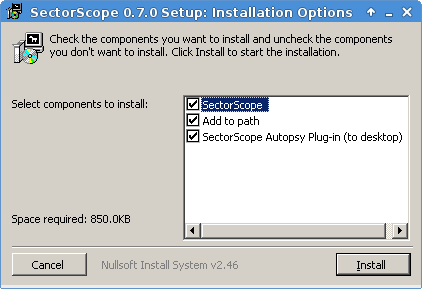
\includegraphics[scale=.4]{screenshots/installer}\\

\subsubsection{Installing on Linux or Mac}
\begin{itemize}
\item Download \sscope files from the \verb+.zip+ file under \url{http://digitalcorpora.org/downloads/sectorscope/}.
\item Unzip  the downloaded \verb+.zip+ file to extract \sscope.
\item Copy these unzipped files to a directory where you can run them or set your \verb+PATH+ variable to find them. For example create directory \verb+local/bin+ in your home directory and copy the files there. Then add the following text to your \verb+$HOME/.bash+ file and then close and reopen your command window so that these tools can be found:

\begingroup
\footnotesize
\begin{Verbatim}[fontfamily=courier]
# User specific aliases and functions
PATH=$HOME/local/bin:$PATH
\end{Verbatim}
\endgroup
\end{itemize}

\subsubsection{Installing Other Resources}
\sscope requires other resources to run:
\begin{itemize}
\item \textbf{hashdb}\\
\sscope uses \hdb to run scans, ingest block hashes, and read media image bytes.\\

For Windows: download and run the latest \hdb Windows installer available under \url{http://digitalcorpora.org/downloads/hashdb/}. It is named\\
\verb+hashdb-x.y.z-windowsinstallelr.exe+ where x.y.z is the latest version.\\

For Linux and Mac: download and build \hdb as described in the \hdb Users Manual available at \url{http://digitalcorpora.org/downloads/hashdb/} or on the \hdb Wiki at \url{https://github.com/NPS-DEEP/hashdb/wiki/Installing-hashdb}.

\item \textbf{Python}\\
\sscope requires Python2.7 or Python3. Please see \url{https://www.python.org/downloads/} to install Python.
\item \textbf{TSK}\\
Although TSK is required for generating media image annotations, \sscope can run without it. To support media image annotations, please install TSK executables and libraries from \url{http://www.sleuthkit.org/sleuthkit/download.php} and set your \verb+PATH+ variable to include the installed \verb+bin+ directory.
\item \textbf{Autopsy}\\
If you would like to run \sscope from \aut, please also install \aut, \url{http://www.sleuthkit.org/autopsy}. Note that the \sscope \aut plug-in module must also be installed and configured, described below.
\end{itemize}

\subsubsection{Installing the \sscope \aut Plug-in Module}
\label{installingNBM}
The \sscope Windows installer installs the \verb+.nbm+ \sscope \aut plug-in module onto the desktop. Please follow these steps to install this module into the \aut workflow:
\begin{enumerate}
\item Open \aut. From the \aut menu, select \verb+Tools | Plugins+.
\item Open the \verb+Downloaded+ tab and click the \verb+Add Plugins...+ button.
\item From the \verb+Add Plugins+ window, navigate to the \verb+.nbm+ module file that was installed onto the desktop, and open it. It may be at \verb+C:\Users\Public\Public Desktop+.
\item Click \verb+Install+ and follow the wizard.
\end{enumerate}

\subsubsection{Configuring the \sscope \aut Plug-in Module}
\label{configuringNBM}
The path to the \hdb database must be configured:
\begin{enumerate}
\item Start a new case, \verb+File | New Case...+, fill in the Case Information fields, and click Next.
\item Fill in Case Information and click Finish.
\item For \verb+Add Data Source+ (1 of 3), put in a media image for \aut to process and click \verb+Next+.
\item For \verb+Add Data Source+ (2 of 3), select checkboxes as desired, then click on \verb+SectorScope+ text to configure the path to your \hdb database to scan against. Currently a file chooser is not available, so please type in the full path, for example: \verb+C:\Users\me\my_hashdb.hdb+. Click \verb+Next+.
\item For \verb+Add Data Source+ (3 of 3) click \verb+Finish+. When the \sscope module begins processing, \aut will display "NPS-SectorScope ..." as \hdb runs, which may take up to several hours. Unfortunately, \hdb progress is not currently indicated. For diagnostics: please see text in the generated log file and in the generated \verb+stderr_hashdb.txt+ file and try running the scan directly from \sscope.\\
\end{enumerate}

\subsection{Starting \sscope}
To open \sscope, type the following on the command line:
\begin{Verbatim}[commandchars=\\\{\}]
\verbbf{sectorscope.py}
\end{Verbatim}
If desired, \sscope may be opened with alternate parameters so that it starts with a scan dataset. Type \verb+sectorscope.py -h+ for help on options.\\

\sscope runs from \aut. To start \sscope from \aut, click the \verb+SectorScope+ property in the \aut window.

\section{Working with \sscope}
\subsection{Managing Massive Datasets}
Block hash scans can produce a large amount of matches. \sscope provides filters to highlight and ignore data:
\begin{itemize}
\item \textbf{Highlight Sectors and Hashes}\\
Entire sectors or individual hashes may be highlighted.
\item \textbf{Ignore Sectors and Hashes}\\
Entire sectors or individual hashes may be ignored.
\item \textbf{Ignore Entropy Range}\\
All hashes from blocks below or above given entropy values may be ignored.
\item \textbf{Ignore Maximum Duplicate Hashes}\\
All hashes with a duplicates count above a maximum may be ignored.
\item \textbf{Ignore Auto-filter Labeled Hashes}\\
All hashes marked with a block label may be ignored.
\end{itemize}
\sscope is able to provide filtering by using block and source information stored in the \hdb database. Specifically:
\begin{itemize}
\item \textbf{Block Entropy}\\
Low entropy blocks are frequently nonprobative.
\item \textbf{Block Label}\\
\hdb generates block labels for blocks possessing specific characteristics. \hdb generates several block labels. Defining effective block labels is an area of research.
\item \textbf{Source Size}\\
The source size is used to calculate the percentage of a source that was matched.
\item \textbf{Count}\\
The count of matches for a block and the sub-count of matches contributed by each source for a block are used to indicate how common a block is.
\item \textbf{Source Label}\\
Source labels may be used to infer expected entropy values. \hdb and \sscope do not use this information. This is an area of research.
\end{itemize}

\subsection{Scan Files}
Scan files contain the information about the blocks in a media image that match 
blacklist blocks in a block hash database. \sscope contains the interfaces necessary for creating \hdb databases, creating scan files by scanning media images, and viewing match information contained in scan files.

\subsection{Histogram Graph}
The histogram graph shows a histogram of frequencies of matched hashes along a scanned media image. Controls in the user interface allow the user to pan and zoom the graph, highlight or ignore regions of the histogram, correlate matches with source files, and export sectors of the media image.

\subsection{Media Image Annotations}
\label{annotations}
\sscope displays media annotations below the histogam bars. The following annotation types are currently supported:
\begin{itemize}
\item Disk partition information obtained by running the TSK \verb+mmls+ command.
\item File system information obtained by running the TSK \verb+fsstat+ command.
\end{itemize}

Annotation entries define the annotation type, the offset and length of the content being annotated, and annotation text. New annotation types may be added in the future.\\

\sscope has the ability to work with sector sizes other than 512 bytes. The TSK tools that \sscope use to produce annotation expect a sector size of 512 bytes. To prevent reporting incorrect units, \sscope will not open annotations when the sector size specified when opening a scan is not 512.\\

The first time a scan file is opened by \sscope, \sscope prepares annotation content in a subdirectory next to the scan file named \verb+<scan file>.temp_annotations+. For example if the scan file is named \verb+scanfile.json+, annotations will be generated at \verb+scanfile.json.temp_annotations+. \sscope references information in this subdirectory in order to display annotation content. This subdirectory may be deleted. \sscope will generate it again if it is not there.

\subsection{Source Files}
\sscope shows a list of all sources in a hash database that have hashes in common with the media image scan. Changing filter and range selections affect the source list by removing sources or modifying how much of a source is matched.

\section{\sscope User Interfaces}
\subsection{Main Window}
Here is an example screenshot of the \sscope main window:\\
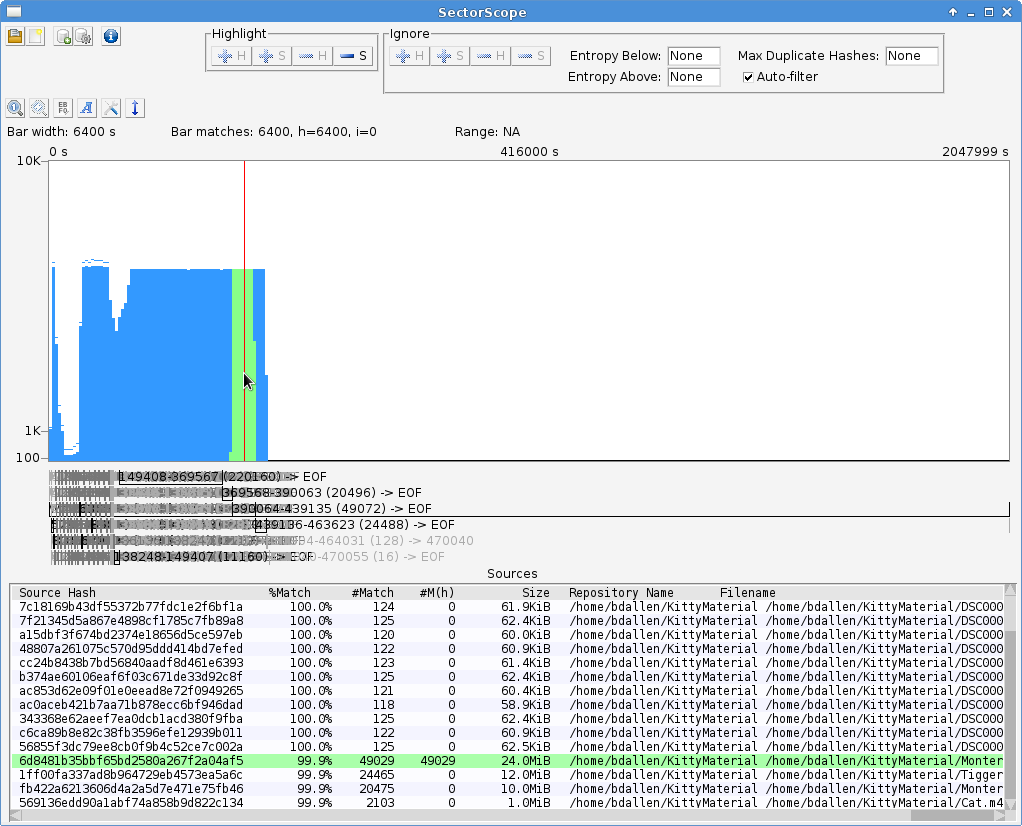
\includegraphics[scale=.4]{screenshots/main_window}\\

\subsection{Menu Controls}
Here are the menu controls:\\
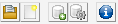
\includegraphics[scale=.4]{screenshots/menu_controls}\\

\subsubsection{Open Scan File}
Use this control to open and view the output of a \hdb scan. Here is the Open Scan File window:\\
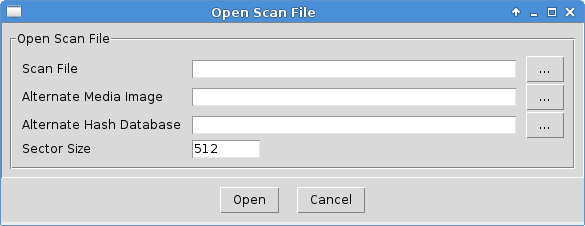
\includegraphics[scale=.4]{screenshots/open_scan_file}\\
\begin{itemize}
\item \textbf{Scan File}\\
When \hdb performs a scan, all matches are placed in this scan file. The scan file also contains the path to the media image scanned and the hash database scanned against. If these paths move, alternate paths may be provided.
\item \textbf{Alternate Media Image}\\
An alternate path to the media image to use if the path in the scan file is incorrect. Keep blank to use the default.
\item \textbf{Alternate Hash Database}\\
An alternate path to the hash database to use if the path in the scan file is incorrect. Keep blank to use the default.
\item \textbf{Sector Size}\\
The sector size for this media, typically 512 bytes. \sscope will display sectors of this size. \sscope will zoom in to this size.
\end{itemize}

\subsubsection{Scan Statistics}
Here is an example of scan statistics:\\
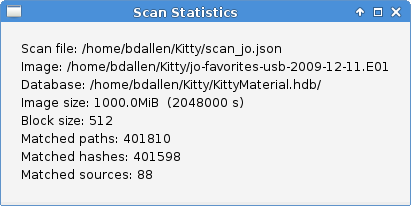
\includegraphics[scale=.4]{screenshots/scan_statistics}\\
Statistics for the opened scan include the path to the scan file, media image, and hash database, the image size, sector size, hash block size, and number of matched paths, hashes, and sources.

\subsubsection{Ingest}
Here is the \sscope Ingest window:\\
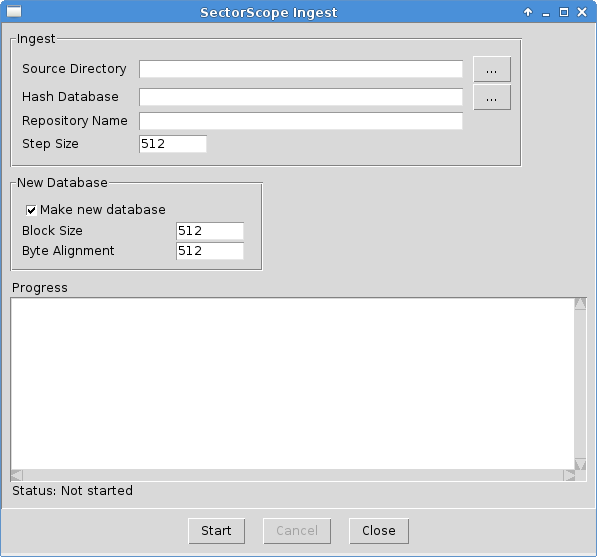
\includegraphics[scale=.4]{screenshots/ingest}\\
Use this window to ingest files or media images into a hash database.
\begin{itemize}
\item \textbf{Source Directory}\\
The path to the source files to ingest recursively from.
\item \textbf{Hash Database}\\
The path to the hash database to import block hashes into.
\item \textbf{Repository Name}\\
The repository name to associate the imported sources with. Leave blank to use the default, which is the source directory path.
\item \textbf{Step Size}\\
The step size to move along while calculating block hashes. The byte alignment must be compatible with the step size, specifically, byte alignment must be divisible by step size.
\item \textbf{Make New Hash Database}\\
If this is selected, a new database will be created instead of using an existing databases. The new database will be created with the following:
  \begin{itemize}
  \item \textbf{Block Size}\\
  The block size to use for calculating the block hash.
  \item \textbf{Byte Alignment}\\
  An optimization parameter, typically the smaller of the block size and the step size.
  \end{itemize}
\end{itemize}

\subsubsection{Scan}
Here is the \sscope Scan Media Image window:\\
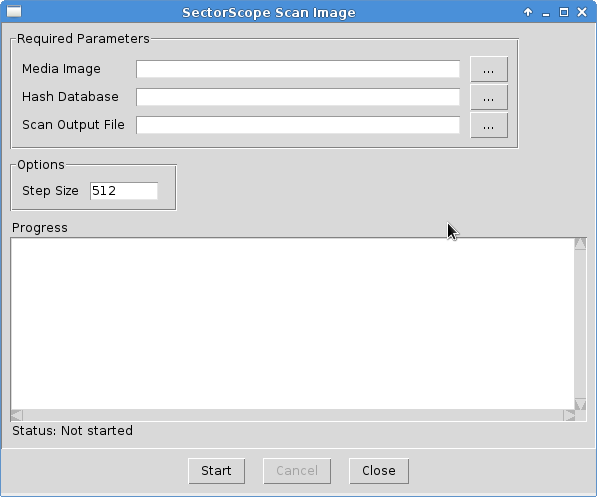
\includegraphics[scale=.4]{screenshots/scan}\\
Use this window to scan a media image for matching block hashes.
\begin{itemize}
\item \textbf{Media Image}\\
The path to the media image to scan.
\item \textbf{Hash Database}\\
The path to the hash database to scan against.
\item \textbf{Sector Size}\\
The sector size for this media, typically 512 bytes. \sscope will display sectors of this size. \sscope will zoom in to this size.
\end{itemize}

\subsubsection{Information}
This button opens a window showing the version of \sscope and \hdb.

\subsection{Highlight and Ignore}
Here is an example view of the highlight and ignore controls:\\
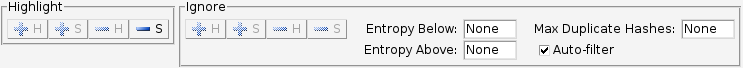
\includegraphics[scale=.4]{screenshots/highlight_and_ignore}\\
These inputs control which hashes and sources are highlighted or ignored in the histogram bar and in the source list. Highlighted items are shown in green. Ignored items are not displayed.
\subsubsection{Highlight}
\begin{itemize}
\item \textbf{+H}\\
Select a range and highlight hashes in this range.
\item \textbf{+S}\\
 Select a range and highlight all sources containing hashes in this range.
\item \textbf{-H}\\
Un-highlight all highlighted hashes.
\item \textbf{-S}\\
Un-highlight all sources.
\end{itemize}

\subsubsection{Ignore}
\begin{itemize}
\item \textbf{+H}\\
Select a range and ignore hashes in this range.
\item \textbf{+S}\\
Select a range and ignore all sources containing hashes in this range.
\item \textbf{-H}\\
Stop ignoring all ignored hashes.
\item \textbf{-S}\\
Stop ignoring all ignored sources.
\item \textbf{Entropy Below}\\
Ignore hashes with an entropy value below this threshold.
\item \textbf{Entropy Above}\\
Ignore hashes with an entropy value above this threshold.
\item \textbf{Max Duplicate Hashes}\\
Ignore hashes matched more than a maximum number of times.
\item \textbf{Auto-filter}\\
Ignore hashes if they have been flagged as potentially non-probative based on experimental entropy calculations.
\end{itemize}

\subsection{Histogram and Media Image Annotation Graph}
Histogram and media image annotations include button controls, cursor controls, graph annotations, and media image annotations:\\
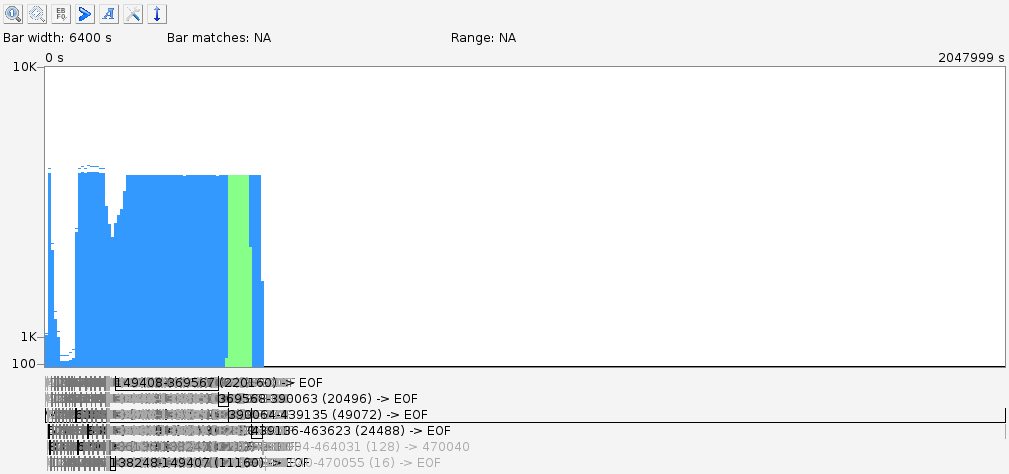
\includegraphics[scale=.4]{screenshots/histogram_and_annotation_graph}\\

\subsubsection{Graph Button Controls}
Here are the histogram and annotation graph button controls:\\

\includegraphics[scale=.4]{screenshots/graph_button_controls}\\
\begin{itemize}
\item \textbf{Zoom to Full Scale}\\
Zoom out so the view spans the entire media iamge.
\item \textbf{Zoom to Range Selection}\\
Zoom in on the selected range to fit the view.
\item \textbf{Show Hex View}\\
Open a window to show the hexadecimal bytes of the block under the cursor.
The following example hex view shows bytes for matched block hash \verb+0x3982...+ at media image offset \verb+0x09c40000+.\\
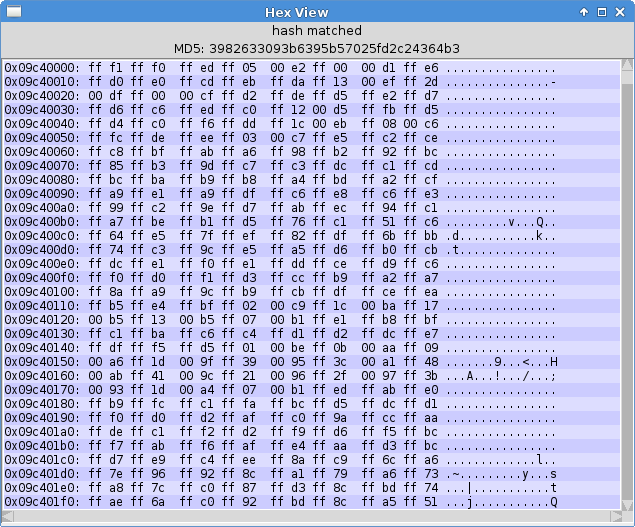
\includegraphics[scale=.4]{screenshots/hex_view}\\
\item \textbf{Export Media Bytes}\\
Open a window to export or append sectors from the media image into a file.\\
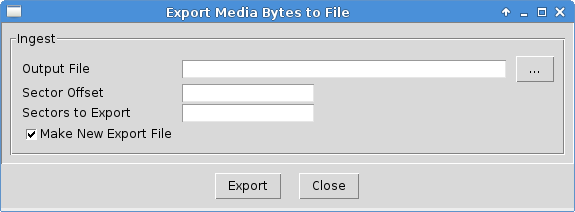
\includegraphics[scale=.4]{screenshots/export_media_bytes}\\
\item \textbf{Manage Annotations}\\
Open a window to enable or disable annotation categories. Here is an example window showing that annotations from disk partitions and file system sectors are enabled:\\
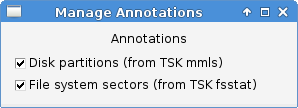
\includegraphics[scale=.4]{screenshots/manage_annotations}\\
  \begin{itemize}
  \item Disk partition annotations are obtained by running the TSK mmls command.
  \item File system sectors are obtained by running the TSK fsstat command.
  \end{itemize}
Please see \textbf{\Autoref{annotations}} for information about media image annotations.
\item \textbf{Toggle offset Units}\\
Toggle the displayed offset units between sectors, decimal bytes, and hexadecimal bytes.
\item \textbf{Toggle Auto-y-axis}\\
Enable or disable auto-y-axis histogram bar scaling.
\end{itemize}

\subsubsection{Histogram}
The histogram graph area shows the frequency of hash matches at given offsets in the media image. Bar width depends on the zoom level. Bar color indicates hashes present within the region of the bar. Blue indicates hashes present. A blue tick above the bar indicates total hashes when hashes are ignored. A green bar indicates highlighted hashes.\\
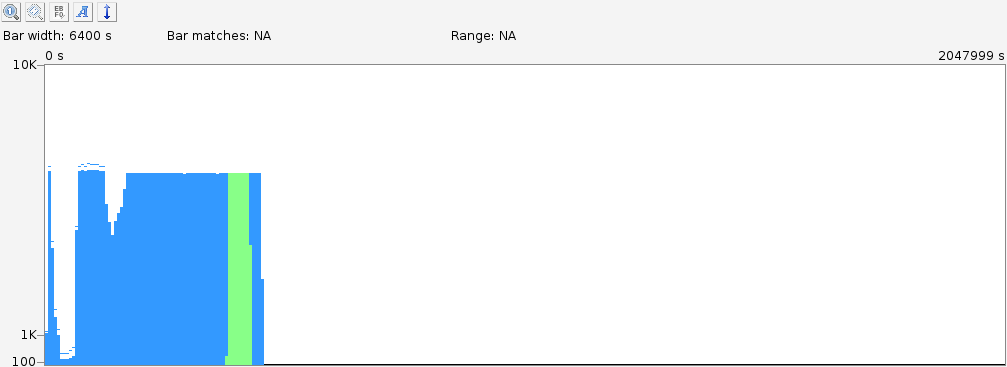
\includegraphics[scale=.4]{screenshots/histogram}\\

\subsubsection{Histogram Bar Annotation}
\begin{itemize}
\item \textbf{Bar width}\\
The number of sectors or bytes spanned by each bar, depending on the offset format.
\item \textbf{Bar matches}\\
The number of matches under the bar that the cursor is hovering over.  Three values are shown: total matches, highlighted matches (h), and ignored matches (i).
\item \textbf{Range}\\
The amount of the media image that the selected range spans.
\item \textbf{Bounds}\\
The first and last offset across the histogram is shown.
\item \textbf{Y-axis scale}\\
The horizontal scale, indicating the number of hash matches required to reach that height. This scale may be toggled between auto-scaling and no scaling.
\end{itemize}

\subsubsection{Histogram Cursor Controls}
Cursor movement, click, drag, and wheel motions manipulate the graph view:
\begin{itemize}
\item Move the mouse to position the cursor. Enable hex view to see the bytes under the cursor.
\item Drag the mouse to select a range. Zoom to expand the graph to the selected range. Ignore or highlight hashes or sources in this selected range.
\item Right-click drag to pan the graph.
\item Roll the wheel to zoom in and out.
\end{itemize}

\subsubsection{Media Image Annotation Graph}
Here is an example view of a media image annotation graph:\\
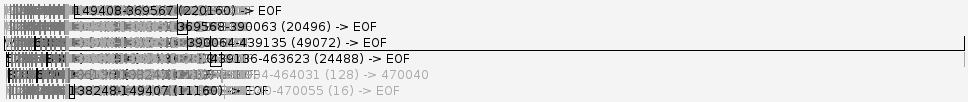
\includegraphics[scale=.4]{screenshots/annotations}\\
Disk partitions and file system sectors are shown. They run over the top of each other because the histogram view is fully zoomed out and there are so many annotations present. To help preserve readability, only annotations that refer to a range that spans a whole histogram bar or more are shown in black, annotations that span less than one histogram bar in width are shown in gray, and annotations that span less than one tenth of a histogram bar are shown in light gray.\\

Please see \textbf{\Autoref{annotations}} for information about media image annotations.

\subsection{Source Table}
Here is an example view of the source table:\\
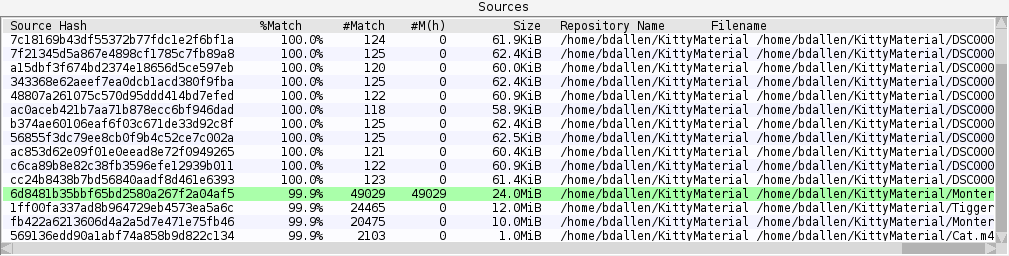
\includegraphics[scale=.4]{screenshots/source_table}\\

\subsubsection{Source Table Contents}
The source table shows information about sources in the hash database that have hashes in common with the media image scan. For each source shown, this information includes the source file hash, how much of the file matched, the file size, and one repository name, filename pair matching this file hash.\\

The set of sources and the percent matched depend on the range selection in the histogram view and filter settings:
\begin{itemize}
\item If a range is not selected in the histogram view, all matched sources are shown except for sources that are filtered as ignored and sources where all matched hashes are filtered as ignored..
\item If a range is selected in the histogram view, only sources with hashes in this range may be shown.
\item If all the hashes that match a source are ignored, the source will not be shown.
\item If some of the hashes that match a source are ignored, the source will be shown, but the percent matched value will be lower.
\item If all the hashes that match a source are ignored, the source will not be shown.
\end{itemize}
Rows in the source table contain the following information:
\begin{itemize}
\item \textbf{Source Hash}\\
The hash hexcode of the source file.
\item \textbf{\%Match}\\
The percent of this source that was matched by the scan.
\item \textbf{\#Match}\\
The number of matches matched by the scan.
\item \textbf{\#M(h)}\\
The number of matches that are highlighted.
\item \textbf{Size}\\
The size of the source file matched.
\item \textbf{Repository Name}\\
A repository name associated with this source file.
\item \textbf{Filename}\\
A filename associated with this source file.
\end{itemize}

\subsubsection{Source Table Controls}
\begin{itemize}
\item If a range is selected, only sources with hashes in that range are shown. Otherwise, all hashes are shown.
\item If all hashes of a source are ignored, that source will not be shown.
\item Click on a source to highlight it. It will show up green. Portions of the histogram bars contributed  by that source will show up green. Re-click to un-highlight.
\item Left-click on a source to ignore it. It will be removed from the sources table. Portions of the histogram bars contributed  by that source will be removed. Ignored sources may be un-ignored using the \textbf{-S} Ignore control.
\end{itemize}

\section{Examples}
\subsection{Create and Scan using \sscope}
In this example, we create a blacklist database of block hashes, then scan a media image for matches:

\begin{enumerate}
\item Identify a directory containing your blacklist source data.
In this example, we use the Kitty Material demo source files available at \url{http://digitalcorpora.org/corpora/scenarios/2009-m57-patents/KittyMaterial} and scan for matches in the demo media image available at \url{http://digitalcorpora.org/corpora/scenarios/2009-m57-patents/drives-redacted/jo-favorites-usb-2009-12-11.E01} which contains blacklist block hashes from the Kitty demo:
\item Start \sscope by typing the following at a command prompt:
\begin{Verbatim}[commandchars=\\\{\}]
\verbbf{sectorscope.py}
\end{Verbatim} 
\item Click on the Ingest menu icon 

\includegraphics[scale=.4]{screenshots/ingest_menu_icon}
to open the \sscope Ingest window.
\item Fill in the fields:
  \begin{itemize}
  \item Set Source Directory to the directory containing your blacklist source data.
  \item Set Hash Database to your new hash database.
  \item Set the Repository Name to the name of this case dataset, or leave blank to use the source directory as the repository name.
  \item Use the default step size to ingest along sector intervals.
  \item Keep Make New Hash Database checked since you will not be ingesting block hashes into an existing database.
  \item Use the default block size to calculate sector-sized block hashes.
  \item Use the default byte alignment since the blocks are sector-aligned.
  \end{itemize}
\item Click the \verb+Start+ button to begin the process of ingesting block hashes from files under the source directory. Progress information will be displayed. When done, status will indicate \verb+Done+. Close the window.
\item Click on the scan media image icon

\includegraphics[scale=.4]{screenshots/scan_media_image_icon}
to open the \sscope Scan Media Image window.
\item Fill in the fields:
  \begin{itemize}
  \item Set the path to the media image to be scanned.
  \item Set the path to the newly created hash database.
  \item Set the path to the scan output file that will be generated.
  \item Use the default step size to scan along sector intervals.
  \end{itemize}
\item Click the \verb+Start+ button to begin the process of scanning for matching block hashes. Progress information will be displayed. When done, status will indicate \verb+Done+. Close the window.
\item Click on the Open scanned output icon

\includegraphics[scale=.4]{screenshots/open_scanned_output_icon}
to open the Open Scan File window which opens the scan data into \sscope.
\item Fill in the fields:
  \begin{itemize}
  \item Set the path to newly created scan file.
  \item Leave the alternate media image field blank since the path to the media image defined in the scan file is correct.
  \item Leave the alternate hash database field blank since the path to the hash database defined in the scan file is correct.
  \item Use the default sector size to view sector offsets for 512-byte-sized sectors.
  \end{itemize}
\item Click the \verb+Open+ button to load this scan dataset into \sscope. It can take 30 seconds or more to load large scan datasets. \sscope currently does not show progress during open. Close the window.
\item Manipulate \sscope controls to examine matched data.
\end{enumerate}

\subsection{Scan using \aut}
\begin{enumerate}
\item Obtain a populated hash database and a media image to scan. This example uses the database and media image described in the previous example.
\item Start \aut and select \verb+Add Data Source+ if this window is not already open.
\item In \verb+Add Data Source+ Step 1, select the path to media image \verb+jo-favorites-usb-2009-12-11.E01+ and click \verb+Next+.
\item In \verb+Add Data Source+ Step 2, configure ingest modules, select the SectorScope ingest module and type in the full path to the \verb+kitty_blacklist.hdb+ block hash blacklist database (file chooser capability is not available yet). Deselect other modules as desired. Click \verb+Next+. Autopsy will remember these settings.
\item In \verb+Add Data Source+ Step 3, click finish.
\item When processing completes, click on Reports in the tree on the left to show the Reports table. In the Reports table, click on the \verb+Block Hash Blacklist+ cell to open \sscope.
\end{enumerate}

\section{Alternate Configurations}
\begin{itemize}
\item \textbf{Alternate Hash Algorithm}\\
\sscope calculates MD5 hashes when showing block hash values in the hex view. If your use-case requires a hash algorithm other than MD5, please see source code file \verb+NPS-SectorScope/python/media_hex_window.py+ for instructions on changing this algorithm.
\end{itemize}

\end{document}
